\documentclass{IEEEtran}
\usepackage[margin=1in]{geometry}
\usepackage{amssymb}
\usepackage{enumitem}
\usepackage{amsmath}
\usepackage{graphicx}
\usepackage{caption}
\usepackage{siunitx}
\usepackage{algorithm}
\usepackage{algorithmic}
\usepackage{bbold}
\usepackage{tikz}
\usetikzlibrary{calc, shapes, backgrounds}
\title{Developing Feedback-Based Coding Schemes for Stochastic Bit Arival
Times}
\author{Ali Cataltepe\thanks{Thanks to Evan Gunter for suggesting to look at
trees in the first place.}\\ Mentor: Victoria Kostina, Co-mentor: Nian Guo\\
Caltech SURF 2020\vspace{-3em}}
\date{}
\IEEEoverridecommandlockouts
\begin{document}
\maketitle
\begin{abstract}
Error-correcting codes (ECCs) that rely on noiseless feedback have been
studied extensively for decades. However, the most theoretically rigorous
methods in this area do not apply to a causal setting, where the encoder
does not know the entirety of the message they wish to transmit beforehand.
Of particular interest among feedback-based ECCs are those operating on the
Small-Enough-Difference (SED) principle, where the entire vocabulary of
possible messages is deterministically divided into two groups with probability
mass difference less than that of a single message.
The Information Theory Group at
Caltech has developed a causal ECC which assumes predetermined bit arrival
times. In this paper we propose two implementations of a causal ECC for
a setting with uniformly random bit arrival times, performing a natural
grouping of low-probability messages using the tree structure of binary
strings to achieve linear-time performance. Even when it does not
explicitly	
attempt to
meet the SED criterion, this algorithm performs at channel capacity
with fixed message lengths, and stabilizes the leading 90\% of bits of
streamed data from a random plant at bit arrival probabilities up to channel
capacity.
\end{abstract}
\section{Introduction}
A \textit{communications channel} is a channel over which an
agent (an \textit{encoder}) can transmit symbols to another agent
(a \textit{decoder}).
This is typically modeled by the channel taking a symbol from the encoder's
end as input and producing another symbol at the decoder's end as output.
Many communications channels are \textit{noisy}, in that the decoder cannot
know for certain which symbol the encoder has inputted from what they have
received. A common example of such a channel is the
noisy \textit{binary symmetric channel} (BSC), over which either a 0
or a 1 can be sent, with a fixed and known probability that
the transmitted symbol will be the inverse of what was sent.

A communications
channel has \textit{noiseless feedback} when the encoder knows for certain
what symbol the decoder has received. A communication channel's
\textit{capacity} is the maximum number of bits of information
which can be conveyed through it per transmission. Simply, this is the
expected value of the inverse of the expected number of transmissions it
would take to
convey a single bit to arbitrary certainty. For a BSC, this value is
$1-H(p)$, where $H$ is the
\textit{Shannon entropy function} and $p$ is the probability
that a bit will be transmitted correctly through the channel. It is
not increased if the channel has feedback~\cite{horsteinseq}.

An \textit{error-correction scheme}
or \textit{error-correcting code}
is any algorithm used to convey information over a noisy communications
channel, with the aim of minimizing the probability of error at the time
transmissions end. Equivalently, this means
maximizing the information conveyed over the channel
per transmission. A setting where an error-correction scheme
is applied is \textit{non-causal} when the entirety
of the message to be transmitted is known by the encoder at the time
the first transmission is made. A setting is \textit{causal}
if the encoder does not know the entirety of the message at the time
they make the first transmission, and the message is revealed to them
over time.

This document provides specifications and empirical results for a
linear-time
solution to the problem setting posed by Guo et al.~\cite{guosed},
developed during the summer of 2020 as part of Caltech's Summer
Undergraduate Research Fellowship program. The accompanying
test code can be found at~\cite{cataltepecausal}.

\section{Background}
Error-correction schemes in binary symmetric channels with feedback have been
studied extensively by Horstein, Waeber, and others~\cite{horsteinseq,
waeberbisection,burnashevestimation}.
However, most theoretical papers with computationally practical algorithms
deal with transmissions in a non-causal
setting, while channels with feedback have the most practical value in real-time
applications, which are almost exclusively causal. Non-causal methods have
the advantage of being able to represent the message to be transmitted as
a point on the interval $[0,1)$. This means
they are able to use the median of
a probability distribution on this interval to easily bisect the vocabulary
of all possible binary strings at each transmission and maximize the
information provided by the encoder's transmissions~\cite{waeberbisection}.
Following Waeber's example~\cite{waeberbisection},
we will call error-correction schemes that
divide the vocabulary of possible messages
into two complementary subsets
``probabilistic bisection algorithms'' (PBAs). We will denote the vocabulary
of possible messages possessed by the encoder at step $i$ as $\mathcal{B}_i$,
and denote the two subsets we divide it into
at any given step as $G_0$ and $G_1$.
Most PBAs seek to minimize the difference in probability mass between $G_0$
and $G_1$.

There has been recent important
theoretical work on PBAs in settings with a finite number of possible
messages, of which causal settings are a subset.
Instead of treating messages as points on a number line,
Naghshvar et al.~\cite{javidiextrinsic} propose a
\textit{smallest-enough-difference} (SED) criterion for an
encoding scheme, which ensures optimality in settings where there is a
finite number of possible messages at the time of each transmission. This
criterion is weaker than finding the true minimum difference in probability
mass between $G_0$ and $G_1$---it merely requires that the difference be
less than or equal to the minimum probability mass of a string in
$\mathcal{B}_i$,
provided the true minimum difference is not larger than this. Previously,
minimizing the probability mass difference between $G_0$ and $G_1$ was an
instance of the Partition problem, which is NP-hard~\cite{karpnp}. However,
using the SED criterion instead, Antonini et al.~\cite{antoninilow}
from the UCLA Communications Systems Laboratory have been able to develop
a quadratic-time algorithm for sending a finite-length message over a BSC
with feedback. While this algorithm rapidly approaches capacity
for a finite blocklength,
it assumes the encoder knows the entirety of its message beforehand, and so
only applies to a non-causal setting. The problem of dividing $G_0$ and $G_1$ in
a causal setting still remains of interest. Achieving SED, let alone minimal
probability mass difference between $G_0$ and $G_1$, is computationally
difficult when $\mathcal{B}_i$ is no longer static.

Placing additional constraints on a causal setting can help sidestep
the difficulty of this requirement.
The Information Theory Group at Caltech has developed a
causal PBA for a setting where the encoder receives new bits
of the message at predetermined times which achieves
capacity on a BSC~\cite{lalithareal}. In this paper, we specify a protocol
for a causal PBA
in a similar setting, but with \textit{uniformly random} bit arrival
times~\cite{guosed} instead of fixed arrival times. Since the
vocabulary of possible messages grows exponentially, it is
important that we avoid doing computations on the entire vocabulary
at once. We detail an
algorithm which takes advantage
of the natural tree structure of $\mathcal{B}_i$ to dramatically reduce
the number of computations required at each step.
This tree-based algorithm is linear-time in message length.

We exhibit experimental results for
both fixed-length messages
and streamed data for the tree-based scheme. We find that
the tree-based scheme shows an exponential
decrease in error for arbitrarily-large fixed proportions of streamed
data for bit-arrival probabilities up to channel capacity. We introduce
a parameter $k$ which adds a constant number of computations per step
to refine $G_0$ and $G_1$, and find that small values of $k$ allow our
algorithm to approach capacity in settings with finite message length.

These results,
combined with its dramatically-reduced computational complexity and motivation
by the structure of $\mathcal{B}_i$, make the tree-based algorithm a
viable implementation for
feedback error correction in a causal setting.
\section{Protocol for a Causal PBA with random bit arrivals}
\label{sec:causalpba}
The specification for this problem setting can also be found in the
paper by Guo et al.~\cite{guosed}.
\subsection{Notation}
We introduce the notations $b[j]$ to denote the $j$-th
character (1-indexed) of a binary string $b$, and $b[j:k]$ to denote
the binary string consisting of the $j$-th character (inclusive) to the
$k$-th character (also inclusive) of $b$ (if $k < j$, then $b[j:k]$ is
the empty string).
We use the function
$\ell(b)$ to denote the length of the binary string $b$. For example,
$b[1:\ell(b)-1]$ denotes the binary string consisting of $b$ without its last
character. We write the values of strings of binary letters
in sans serif, and denote concatenation
by $\boxplus$. For example, $b\boxplus\mathsf{1}$ is an expression for the string
consisting of $b$ with $\mathsf{1}$ appended to the end.
We use $\mathsf{\_}$ to denote the empty string.
As section~\ref{sec:tree} works extensively with subsets
of $\mathcal{B}_i$ grouped by prefix, we use
$\mathcal{B}_i(b)$ to denote the subset of $\mathcal{B}_i$
that is all strings that have the binary string $b$ as a prefix,
including $b$ itself. So, $\mathcal{B}_i(\mathsf{010})$ consists
of $\mathsf{010}$ and all strings in $\mathcal{B}_i$ that begin
with $\mathsf{010}$. It follows that $\mathcal{B}_i(\mathsf{\_})
=\mathcal{B}_i$.
For a set $B$ of messages and a probability mass function $f$,
we define $f(B):=\sum_{b \in B}f(b)$.
We use the indicator function $\mathbb{1}\{\cdot\}$,
which is $1$ if its argument is true and $0$ otherwise.
\subsection{Description of the problem}
\label{ssec:probdescript}
In our setting, an encoder and a decoder communicate over a BSC
with noiseless feedback
which transmits bits correctly with probability $p \in (\frac{1}{2},1)$.
We denote the binary string the encoder has at step $i$ as $b_i^*$. At
each step, with probability $q \in (0,1)$, the encoder receives a new,
previously-unknown bit and appends it to the end of $b_i^*$. The maximum
length $b_i^*$ will reach is $n$, which can be either a positive integer
or infinity. The parameters $p$, $q$, and $n$ are known to both the encoder
and decoder at the time transmissions begin, which is when the encoder receives
the first bit. At each step, the encoder can transmit a bit, and the decoder
will receive the bit $y_i$, which will match the sent bit with probability $p$.
After this, the decoder attempts to produce an estimate for
$b_{i+1}^*$, which we will denote as $x_{i+1}$.
\subsection{Reduced average channel capacity}
The encoder cannot transmit more bits of information than $\ell(b_i^*)$ over
the BSC. However, they also cannot transmit more bits of information than
$(1-H(p))\cdot i$, which is simply the upper bound of channel capacity multiplied
by the total number of transmissions.
We can model the probability mass function for $\ell(b_i^*)$ as a modified
Poisson distribution where $\mathbb{E}(\ell(b_i^*))=i\cdot q$, where the domain
ends at $\ell(b_i^*)=\min(i,n)$, which has all the remaining probability mass.
Designate this function
\begin{multline}
m_i:\{1,\dots,\min(i,n)\} \to (0,1)\\
	m_i(l) = \begin{cases}
	\mathrm{Pois}(i\cdot q)(l) & l < \min(i,n) \\
        \mbox{\scriptsize $1-\mathrm{CDF}(\mathrm{Pois}(i\cdot q))(\min(i,n))$}
          & l= \min(i,n)
	\end{cases}.
\end{multline}
Now, we
define the probability mass function
\begin{multline}
  \mbox{\scriptsize $t_i: \{1,\dots,\lfloor (1-H(p)) \cdot i\rfloor, (1-H(p))\cdot i\} \to (0,1)$}\\
t_i(l) = \begin{cases}
	m(l) & l \leq \lfloor (1-H(p)) \cdot i\rfloor\\
        \mbox{\scriptsize $1-\mathrm{CDF}(m)((1-H(p))\cdot i)$}
        & l = (1-H(p))\cdot i
\end{cases}.
\end{multline}
This is the probability mass function
of the number of bits of information the encoder will be able to transmit by
step $i$. We define the streaming capacity $c_s(i)$ as the mean of the
probability mass function $t_i$ at step $i$, divided by $i$. Finally, to
accommodate the finite-$n$ case for this setting, we define our new capacity,
\begin{equation}
c(p,q,i,n)=(1-H(p))m_i(n)+c_s(i)(1-m_i(n)).
\end{equation}
This reflects that the channel's effective capacity goes back to $1-H(p)$ in
cases where the encoder has determined all the bits they need to transmit.
To determine the upper bound on rate, we then define the function
\begin{equation}
R(p,q,n)= \frac{n}{\inf_{\mathbb{Z}^+}\{\tau \mid n \leq
\sum_{i=1}^{\tau}c(p,q,i,n) \}}.
\end{equation}
We plot this function alongside our rate measurements to provide a more accurate
upper bound on performance.
\subsection{Requirements of a causal PBA}
\label{ssec:reqs}
At each step $i \leq n$, let the vocabulary $\mathcal{B}_i$
denote the set of all binary strings up to length $i$. For further steps,
the vocabulary is always $\mathcal{B}_n$. The decoder maintains a probability
mass function $f_i\colon\mathcal{B}_i \to (0,1)$,
which is determined solely by
$p$, $q$, $n$, and the bits received by the decoder
up to step $i$\footnote{The range of $f_i$ excludes
$0$ and $1$ because the oracle is imperfect.}. This
function is therefore known to the encoder as well.
\subsubsection{Division of the vocabulary}
The decoder must use a deterministic process, depending on the algorithm
used, to divide $\mathcal{B}_i$ into
complementary, nonempty subsets $G_0$ and $G_1$ which satisfy some programmatic
bound on $|f_i(G_0)-f_i(G_1)|$, ideally minimizing it.
\subsubsection{Posterior update of $f_i$}
The encoder, who knows which of $G_0$ or $G_1$ contains $b_i^*$, sends
a 0 if it is in $G_0$ and a 1 otherwise. Upon receiving the bit $y_i$,
the decoder constructs the posterior probability mass function
$f_i'\colon \mathcal{B}_i\to(0,1)$
from $f_i$ using
Bayes' rule.
Define coefficients
$h_0$ and $h_1$ as follows:
\begin{align}
h_{y_i} &=\frac{p}{pf_i(G_{y_i})+(1-p)f_i(G_{\bar{y}_i})}\\
h_{\bar{y}_i} &= \frac{1-p}{pf_i(G_{y_i})+(1-p)f_i(G_{\bar{y}_i})}.
\end{align}
We define $f_i'$ so that
$f_i'(b)=h_0f_i(b)$ is true for $b \in G_0$, and $f_i'(b)=h_1f_i(b)$ is
true for $b \in G_1$.
\subsubsection{Calculating $f_{i+1}$}
Lastly, the updated probability mass function must be used to construct
the prior probability function for the next step, taking into account the
arrival of a new bit with probability $q$.

For strings $b \in \mathcal{B}_{i+1}\setminus\mathcal{B}_i$ of length
$i+1$,
\begin{equation}
f_{i+1}(b)=\frac{q}{2}f_i'(b[1:\ell(b)-1]).
\end{equation}
For strings $b \in \{0,1\}$,
\begin{equation}
f_{i+1}(b)= (1-q)f_i'(b).
\end{equation}
For strings $b \in \mathcal{B}_i\setminus\{0,1\}$:
\begin{equation}
f_{i+1}(b)=(1-q)f_i'(b)+\frac{q}{2}f_i'(b[1:\ell(b)-1]).
\end{equation}

For $i \geq n$, the vocabulary stops growing, so $\mathcal{B}_{i+1}$
is the same as $\mathcal{B}_i=\mathcal{B}_n$.
The update process for $b \in \{0,1\}$ remains the same
and the process for $b \in \mathcal{B}_{n-1}\setminus\{0,1\}$ is the same
as it is for strings in $b \in \mathcal{B}_i\setminus\{0,1\}$. The process
for strings of length $n$, however, is
\begin{equation}
f_{i+1}(b) = \frac{q}{2}f_i'(b[1:\ell(b)-1])+f_i'(b).
\end{equation}

After calculating $f_{i+1}$, the decoder produces $x_{i+1}$, which is usually
the mode.
\subsubsection{Halting and decoding for finite $n$}
Halting and decoding occurs for finite $n$ when $i \geq n$ and
$f_i(x_i) \geq 1-\epsilon$, where
$\epsilon$ is an arbitrarily chosen small value. The current
estimate $x_i$ is now considered
to be the decoder's final guess for what $b_i^*$ is.
\begin{figure*}
\centering
\begin{tabular}{cccc}
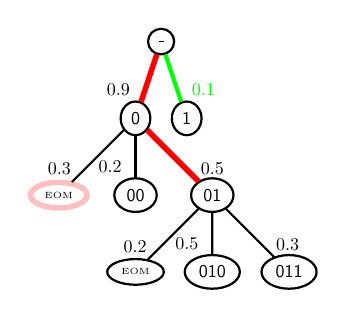
\begin{tikzpicture}[
    scale = 0.65, transform shape, thick,
    every node/.style = {draw, ellipse, minimum size = 5mm}, 
    grow = down,  % alignment of characters
    level 1/.style = {sibling distance=1cm},
    level 2/.style = {sibling distance=1.5cm}, 
    level 3/.style = {sibling distance=1.5cm},
    level 4/.style = {sibling distance=2cm},
    level distance = 1.5 cm
  ]
		\node (Start){$\mathsf{\_}$}
		child {   node (0) {$\mathsf{0}$}
		child {node[draw=pink, solid, line width=2pt]
		(0term) {\tiny {EOM}} }
		child { node  (00) {$\mathsf{00}$}}
		child { node (01) {$\mathsf{01}$}
		child {node (01term) {\tiny{EOM}}}
		child {node (010)
			{$\mathsf{010}$}}
		child {node (011) {$\mathsf{011}$}}
	}
	}
		child {   node (1) {$\mathsf{1}$}};

  % Labels
  \begin{scope}[nodes = {draw = none}]
    \path[draw=red, solid, line width=2pt] (Start)-- (0)
	  node [near end, left]  {$0.9$};
    \path (0)     -- (00) node [near end, left]  {$0.2$};
    \path[draw=red,solid,line width=2pt] (0)   -- (01)
	  node [near end, right] {$0.5$};
    \path (0)     -- (0term) node [near end, left] {$0.3$};
    \path (01)   -- (010)
	  node [near end, left] {$0.5$};
    \path (01) -- (01term) node [near end, left] {$0.2$};
    \path (01) --(011) node [near end, right] {$0.3$};
    \path[draw=green, solid, line width=1.5pt]
	  (Start) -- (1) node [near end, right] {$\color{green}{0.1}$};
  \end{scope}

\end{tikzpicture}

&
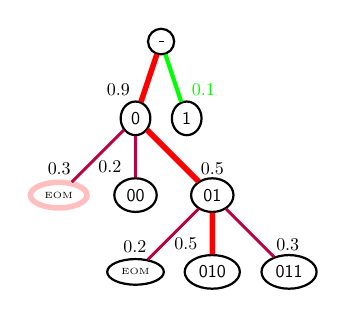
\begin{tikzpicture}[
    scale = 0.65, transform shape, thick,
    every node/.style = {draw, ellipse, minimum size = 5mm}, 
    grow = down,  % alignment of characters
    level 1/.style = {sibling distance=1cm},
    level 2/.style = {sibling distance=1.5cm}, 
    level 3/.style = {sibling distance=1.5cm},
    level 4/.style = {sibling distance=2cm},
    level distance = 1.5 cm
  ]
		\node (Start){$\mathsf{\_}$}
		child {   node (0) {$\mathsf{0}$}
		child {node[draw=pink, solid, line width=2pt]
		(0term) {\tiny {EOM}} }
		child { node  (00) {$\mathsf{00}$}}
		child { node (01) {$\mathsf{01}$}
		child {node (01term) {\tiny{EOM}}}
		child {node (010)
			{$\mathsf{010}$}}
		child {node (011) {$\mathsf{011}$}}
	}
	}
		child {   node (1) {$\mathsf{1}$}};

  % Labels
  \begin{scope}[nodes = {draw = none}]
    \path[draw=red, solid, line width=2pt] (Start)-- (0)
	  node [near end, left]  {$0.9$};
    \path[draw=purple, solid, line width=1pt] (0) -- (00)
	  node [near end, left]  {$0.2$};
    \path[draw=red,solid,line width=2pt] (0)   -- (01)
	  node [near end, right] {$0.5$};
    \path[draw=purple, solid, line width=1pt] (0) -- (0term)
	  node [near end, left] {$0.3$};
    \path[draw=red,solid,line width=2pt] (01)   -- (010)
	  node [near end, left] {$0.5$};
    \path[draw=purple, solid, line width=1pt] (01) -- (01term)
	  node [near end, left] {$0.2$};
    \path[draw=purple, solid, line width=1pt] (01) --(011)
	  node [near end, right] {$0.3$};
    \path[draw=green, solid, line width=1.5pt]
	  (Start) -- (1) node [near end, right] {$\color{green}{0.1}$};
  \end{scope}

\end{tikzpicture}
&
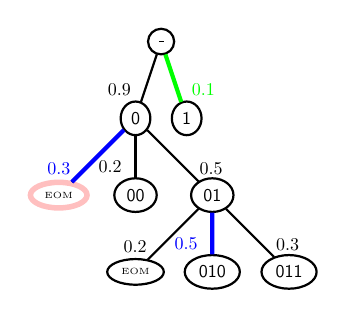
\begin{tikzpicture}[
    scale = 0.65, transform shape, thick,
    every node/.style = {draw, ellipse, minimum size = 5mm}, 
    grow = down,  % alignment of characters
    level 1/.style = {sibling distance=1cm},
    level 2/.style = {sibling distance=1.5cm}, 
    level 3/.style = {sibling distance=1.5cm},
    level 4/.style = {sibling distance=2cm},
    level distance = 1.5 cm
  ]
		\node (Start){$\mathsf{\_}$}
		child {   node (0) {$\mathsf{0}$}
		child {node[draw=pink, solid, line width=2pt]
		(0term) {\tiny {EOM}} }
		child { node  (00) {$\mathsf{00}$}}
		child { node (01) {$\mathsf{01}$}
		child {node (01term) {\tiny{EOM}}}
		child {node (010)
			{$\mathsf{010}$}}
		child {node (011) {$\mathsf{011}$}}
	}
	}
		child {   node (1) {$\mathsf{1}$}};

  % Labels
  \begin{scope}[nodes = {draw = none}]
    \path (Start)-- (0)
	  node [near end, left]  {$0.9$};
    \path (0)     -- (00)
	  node [near end, left]  {$0.2$};
    \path (0)   -- (01)
	  node [near end, right] {$0.5$};
    \path[draw=blue, solid, line width=1.5pt] (0)     -- (0term)
	  node [near end, left] {$\color{blue}{0.3}$};
    \path[draw=blue, solid, line width=1.5pt] (01)   -- (010)
	  node [near end, left] {$\color{blue}{0.5}$};
    \path (01) -- (01term)
	  node [near end, left] {$0.2$};
    \path (01) --(011)
	  node [near end, right] {$0.3$};
    \path[draw=green, solid, line width=1.5pt]
	  (Start) -- (1)
	  node [near end, right] {$\color{green}{0.1}$};
  \end{scope}

\end{tikzpicture}
&
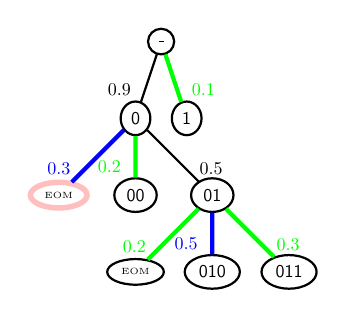
\begin{tikzpicture}[
    scale = 0.65, transform shape, thick,
    every node/.style = {draw, ellipse, minimum size = 5mm}, 
    grow = down,  % alignment of characters
    level 1/.style = {sibling distance=1cm},
    level 2/.style = {sibling distance=1.5cm}, 
    level 3/.style = {sibling distance=1.5cm},
    level 4/.style = {sibling distance=2cm},
    level distance = 1.5 cm
  ]
		\node (Start){$\mathsf{\_}$}
		child {   node (0) {$\mathsf{0}$}
		child {node[draw=pink, solid, line width=2pt]
		(0term) {\tiny {EOM}} }
		child { node  (00) {$\mathsf{00}$}}
		child { node (01) {$\mathsf{01}$}
		child {node (01term) {\tiny{EOM}}}
		child {node (010)
			{$\mathsf{010}$}}
		child {node (011) {$\mathsf{011}$}}
	}
	}
		child {   node (1) {$\mathsf{1}$}};

  % Labels
  \begin{scope}[nodes = {draw = none}]
    \path (Start)-- (0)
	  node [near end, left]  {$0.9$};
    \path[draw=green, solid, line width=1.5pt] (0)     -- (00)
	  node [near end, left]  {$\color{green}{0.2}$};
    \path (0)   -- (01)
	  node [near end, right] {$0.5$};
    \path[draw=blue, solid, line width=1.5pt] (0)     -- (0term)
	  node [near end, left] {$\color{blue}{0.3}$};
    \path[draw=blue, solid, line width=1.5pt] (01)   -- (010)
	  node [near end, left] {$\color{blue}{0.5}$};
    \path[draw=green, solid, line width=1.5pt] (01) -- (01term)
	  node [near end, left] {$\color{green}{0.2}$};
    \path[draw=green, solid, line width=1.5pt] (01) --(011)
	  node [near end, right] {$\color{green}{0.3}$};
    \path[draw=green, solid, line width=1.5pt]
	  (Start) -- (1)
	  node [near end, right] {$\color{green}{0.1}$};
  \end{scope}

\end{tikzpicture}
\\
(a) & (b) & (c) & (d)
\end{tabular}
	\captionof{figure}{An example of how the tree-based algorithm divides
	$G_0$ and $G_1$ when $\lceil q\cdot i\rceil = 3$ and $k=1$.
	The label $v$ on each node indicates a binary prefix.
	The value on the edge leading to $v\boxplus\mathsf{1}$ is
	$\frac{f_i(\mathcal{B}_i(v\boxplus\mathsf{1}))}{f_i(\mathcal{B}_i(v))}$,
	the value on the edge leading to $v\boxplus\mathsf{0}$ is
	$\frac{f_i(\mathcal{B}_i(v\boxplus\mathsf{0}))}{f_i(\mathcal{B}_i(v))}$,
	and the value on the edge leading to ``EOM'' is
	$\frac{f_i(v)}{f_i(\mathcal{B}_i(v))}$. Red indicates the path that has
	been traversed by the program, blue indicates edges added to $G_0$,
	and green indicates edges added to $G_1$. Purple indicates edges leading
	to subtrees examined in $K$. The node corresponding to the
	decoder's current estimate is circled in pink.}
	\label{fig:corpustree}
\end{figure*}

\section{Tree-based algorithm}
\label{sec:tree}
\subsection{Representing $f_i$ using a ternary
tree}
\label{ssec:treerep}
The space of all binary strings up to a certain length has a natural tree
structure, illustrated in Figure~\ref{fig:corpustree}, where
each node is associated with a binary prefix. The
root node is associated with the empty string $\mathsf{\_}$ and
each string $b$ has two children associated with
$b\boxplus\mathsf{0}$ and $b\boxplus\mathsf{1}$. The probability
mass function $f_i$ can
be represented using this tree, without having to compute individual
probabilities for each string in $\mathcal{B}_i$ upon modification
by the posterior and prior-update processes described
in section~\ref{ssec:reqs}. Each node $b$ has
three downward-leading edges that store conditional probabilities
derived from $f_i$:
\begin{itemize}
	\item The \textit{termination-edge} stores the probability
		the decoder assigns to $b_i^*=b$ given that
		$b_i^* \in \mathcal{B}_i(b)$. This quantity
		is expressible as
		$\frac{f_i(b)}{f_i(\mathcal{B}_i(b))}$. The
		termination-edge leads to an empty child
		node.
	\item The \textit{one-edge} stores the probability
		the decoder assigns to $b_i^*
		\in\mathcal{B}_i(b\boxplus \mathsf{1})$ given that
		$b_i^* \in \mathcal{B}_i(b)$. This
		quantity is expressible as
		$\frac{f_i(\mathcal{B}_i(b\boxplus \mathsf{1}))}
		{f_i(\mathcal{B}_i(b))}$. The one-edge
		leads to the node associated with
		the string $b\boxplus \mathsf{1}$.
	\item The \textit{zero-edge} stores the probability
		the decoder assigns to $b_i^*
		\in\mathcal{B}_i(b\boxplus \mathsf{0})$ given that
		$b_i^* \in \mathcal{B}_i(b)$. This
		quantity is expressible as
		$\frac{f_i(\mathcal{B}_i(b\boxplus \mathsf{0}))}
		{f_i(\mathcal{B}_i(b))}$. The zero-edge
		leads to the node associated with
		the string $b\boxplus \mathsf{0}$.
\end{itemize}
Suppose we want to find the value of $f_i(b)$ for some
$b \in \mathcal{B}_i$. We can
start from the root node and follow each edge that will take us
towards the termination-edge of the node associated with $b$. 
If we keep a cumulative product of the values on all
the edges we traverse, we find that 
\begin{equation}
f_i(\mathcal{B}_i(b[1])) \cdot \frac{f_i(\mathcal{B}_i(b[1:2]))}
{f_i(\mathcal{B}_i(b[1]))} \cdots
\frac{f_i(b)}
{f_i(\mathcal{B}_i(b))}=f_i(b)
\end{equation}
because the denominators at each step cancel. Therefore, determining
the value of $f_i(b)$ and $f_i(\mathcal{B}_i(b[1:k]))$ for all $k$
such that $k < \ell(b)$ will take a number of total operations
that scales linearly with $\ell(b)$.

\subsection{Prior-update protocol}
\label{ssec:treeprior}
Suppose for some binary string
$b$ such that $\ell(b) < n$, we know
the value $\frac{f_s'(b)}{f_s'(\mathcal{B}_s(b))}$, the value
$\frac{f_s'(\mathcal{B}_s(b\boxplus \mathsf{1}))}{f_s'(\mathcal{B}_s(b))}$,
and the value
$\frac{f_s'(\mathcal{B}_s(b\boxplus \mathsf{0}))}{f_s'(\mathcal{B}_s(b))}$
for some step $s$ such that $s < i$. If $\mathcal{B}_j(b)$
has been contained in a single bin for all steps $j$ such that
$s< j \leq i$, then the value of $\frac{f_i(b)}{f_i(\mathcal{B}_i(b))}$
can be calculated in one of two different ways.
\subsubsection{Complex approximation}
We can calculate $\frac{f_j(b)}{f_j(\mathcal{B}_j(b))}$ for
	each intermediate step $j$ such that $s<j\leq i$ via
	the expression
\begin{multline}
\frac{f_j(b)}{f_i(\mathcal{B}_j(b))} = \frac{(1-q)f_{j-1}'(b)+\frac{q}{2}
f_{j-1}'(b[1:\ell(b)-1])}{f_{j-1}'(\mathcal{B}_{j-1}(b))
+\frac{q}{2}f_{j-1}'(b[1:\ell(b)-1])}\\
=\frac{(1-q)\frac{f_{j-1}'(b)}{f_{j-1}'(\mathcal{B}_{j-1}(b))}+
\frac{q}{2}\frac{f_{j-1}'(b[1:\ell(b)-1])}{f_{j-1}'(\mathcal{B}_{j-1}(b))}}
{1+\frac{q}{2}\frac{f_{j-1}'(b[1:\ell(b)-1])}{f_{j-1}'(\mathcal{B}_{j-1}(b))}}.
\label{eqn:complexapprox}
\end{multline}
For $j = s+1$, we know the requisite ratios of $f_s'$ and can calculate
Equation~\ref{eqn:complexapprox} exactly.
For $j > s+1$, we can reliably replace the posterior probability
mass function with the prior probability mass function, since if a node
has not been scrutinized by the algorithm for some number of intermediate
steps, it was contained within a single bin with high probability.
\\ \\
We can calculate the term
$\frac{f_{j-1}(b[1:\ell(b)-1])}{f_{j-1}(\mathcal{B}_{j-1}(b))}$ using
\begin{equation}
\frac{f_{j-1}(b[1:\ell(b)-1])}{f_{j-1}(\mathcal{B}_{j-1}(b[1:\ell(b)-1]))}
\frac{f_{j-1}(\mathcal{B}_{j-1}(b[1:\ell(b)-1]))}
{f_{j-1}(\mathcal{B}_{j-1}(b))}.
\end{equation}
To keep this computation self-contained to the node, we approximate
the term as $\frac{f_i(b[1:\ell(b)-1])}{f_i(\mathcal{B}_i(b))}$, so we
only need to know the values of $f_i$ over the parent node at step $i$. If
we attempted the full, this would require keeping track of all
prior values of the variable for all $b$, which would prove infeasible for
memory conservation and defeat the purpose of the tree representation.
\subsubsection{Simpler approximation}
If we take the term $\frac{q}{2}\frac{f_{j-1}(b[1:\ell(b)-1])}
{f_{j-1}(\mathcal{B}_{j-1}(b))}$ in Equation~\ref{eqn:complexapprox} into
account, we are forced to perform $O(i-s)$ operations as we repeat
the computation that many times. This motivates a lower-complexity
approximation. For positive
numbers $u,w$ such that  $u < 1$, we have it that
\begin{equation}
	\left|\frac{u+w}{1+w}-u\right|=\frac{w-uw}{1+w}
	< (1-u)w.
\end{equation}
This means that we can approximate $\frac{u+w}{1+w} \sim u$ with an upper
bound of $(1-u)w$ on error. This means that if we approximate
\begin{equation}
	\frac{f_j(b)}{f_{j}(\mathcal{B}_j(b))} \sim (1-q) \frac{f_{j-1}(b)}{
		f_{j-1}(\mathcal{B}_{j-1}(b))}
	\label{eqn:stepapprox}
\end{equation}
we will undershoot the true value by at most
\begin{equation}
	\left(1-(1-q)\frac{f_{j-1}(b)}{
		f_{j-1}(\mathcal{B}_{j-1}(b))}\right)\frac{q}{2}
\frac{f_{j-1}(b[1:\ell(b)-1])}
{f_{j-1}(\mathcal{B}_{j-1}(b))}.
\end{equation}
We can set an upper bound on this value via the absolute upper bound of
$f_{j-1}(b[1:\ell(b)-1])$, which is $1-f_{j-1}(\mathcal{B}_{j-1}(b))$,
yielding the expression
\begin{equation}
	\frac{q(1-f_{j-1}(\mathcal{B}_{j-1}))
	(f_{j-1}(\mathcal{B}_{j-1}(b))-(1-q)f_{j-1}(b))}
	{2 f_{j-1}(\mathcal{B}_{j-1}(b))^2}.
\label{eqn:errorbound}
\end{equation}
Since our algorithm stops traversing the tree once it reaches a subtree
with probability mass less than $\frac{1}{2}$, let us assume that
$f_{j-1}(\mathcal{B}_{j-1}(b)) \geq \frac{1}{2}$. This automatically means
that as $\ell(b)$ decreases, the bound set by Equation~\ref{eqn:errorbound}
will become negligibly small since $f_{j-1}(\mathcal{B}_{j-1}(b)) \to 1$.
The upper bound of error within our constraint is reached when
$f_{j-1}(\mathcal{B}_{j-1}(b)) = \frac{1}{2}$, at which point the error
bound becomes bounded by $\frac{q}{2}$, and is likely to be far less than this.
\\ \\
Our key argument in making this approximation is that our algorithm will
depend on greedily traversing the tree by picking the highest-valued edge
at each node. We are thus motivated to introduce a simplification that will
focus more on getting a general ``sense'' of the movement of probability towards
longer strings instead of attempting to get fully-accurate values of $f_i$.
If we apply the approximation in Equation~\ref{eqn:stepapprox} to all the
intermediate steps $j$, we effectively set
\begin{equation}
\frac{f_i(b)}{f_i(\mathcal{B}_i(b))}:=\frac{f_s'(b)}{f_s'(\mathcal{B}_s(b))}
\cdot (1-q)^{i-s}.
\label{eqn:simpapprox}
\end{equation}
This is significantly faster, since a fast exponentiation algorithm will give
it a time complexity of $O(\log (i-s)) $.

After computing $\frac{f_i(b)}{f_i(\mathcal{B}_i(b))}$ by either
of these methods, we define
$d:= \frac{f_s'(b)}{f_s'(\mathcal{B}_s(b))}
-\frac{f_i(b)}{f_i(\mathcal{B}_i(b))}$, the amount of probability
``shifted'' from $b$ to $\mathcal{B}_i(b)\setminus\{b\}$,
and use it to calculate the other two values associated with $b$ in the tree:
\begin{align}
\frac{f_i(\mathcal{B}_i(b\boxplus \mathsf{1}))}
{f_i(\mathcal{B}_i(b))}&=\frac{f_s'(\mathcal{B}_s(b\boxplus \mathsf{1}))}
{f_s'(\mathcal{B}_s(b))}+\frac{d}{2}\\
\frac{f_i(\mathcal{B}_i(b\boxplus \mathsf{0}))}
{f_i(\mathcal{B}_i(b))}&=\frac{f_s'(\mathcal{B}_s(b\boxplus \mathsf{0}))}
{f_s'(\mathcal{B}_s(b))}+\frac{d}{2}.
\end{align}
The lowest value of $s$ at which $\mathcal{B}_s(b) \neq \emptyset$
is when $s=\ell(b)$, at which point it is
true that $\mathcal{B}_s(b) =\{b\}$ and therefore
$\frac{f_s'(b)}{f_s'(\mathcal{B}_s(b))}=1$ (with the other two probabilities
being zero). Therefore, if $b$ has not been evaluated in the tree at
any point up to step $i$,
the values of $f_i$ can be calculated by setting $s=\ell(b)$.

There are two special cases for this calculation.
If $\ell(b) = n$, then $\frac{f_i(b)}{f_i(\mathcal{B}_i(b))}=1$ at all
times because $\mathcal{B}_i(b)=\mathcal{B}_n(b)=\{b\}$. If
$b=\mathsf{\_}$ then $f_i(b)=0$ and the values of
$f_i(\mathcal{B}_i(\mathsf{1}))$ and $f_i(\mathcal{B}_i(\mathsf{0}))$
are thus not affected by the prior-update process, since $d=0$ at
every step. At step $i=1$, we have that $f_1(\mathcal{B}_i(\mathsf{0}))
=f_1(\mathcal{B}_i(\mathsf{1}))=\frac{1}{2}$.

In this formulation, the prior-update process only requires a constant
number of operations to be performed each time a string is looked up
for the first time in a step,
as opposed to a number scaling with $|\mathcal{B}_i|$.

\subsection{Representing $G_0$ and $G_1$}
We represent $G_0$ and $G_1$ using mixed sets of subtrees and individual
strings, where a subtree $\mathcal{B}_i(b)$ is a reference to the edge
storing the value
$\frac{f_i(\mathcal{B}_i(b))}{f_i(\mathcal{B}_i(b[1:\ell(b)-1])))}$, and
an individual string $b$ is a reference to the edge storing the value
$\frac{f_i(b)}{f_i(\mathcal{B}_i(b))}$. This ensures that the posterior
update only requires operations on these edges of interest, instead of
the entirety of $\mathcal{B}_i$.

\subsection{Refining $G_0$ and $G_1$ with the parameter $k$}
We introduce the parameter $k \in \mathbb{N}$, which determines an upper
bound on additional operations done to refine the division of $G_0$ and
$G_1$ to achieve a smaller value of $|f_i(G_0)-f_i(G_1)|$. Once it
initially halts, the algorithm
traverses an extra number of downwards edges equal to $k$ and keeps track of each
tree seen in this process in an ordered set $K$.
Afterwards, it sorts these trees in descending order
by probability mass and adds them sequentially to $G_0$ when an addition would
decrease $|f_i(G_0)-\frac{1}{2}|$. This is a well-known approximation to the
partition problem over $K$ based on a method by
Dantzig~\cite{knapsackapprox}. The algorithm
then adds the remaining trees in $K$
to $G_1$. Since $|K|\sim 2k$ and the time to sort $K$ is $O(|K|\log|K|)$, the
number of operations that $k$ adds to the algorithm depends solely on $k$ and
can be treated as a constant when $k \ll \min(\lceil i\cdot q \rceil,n)$.

\subsection{Updating $G_0$ and $G_1$, and determining $x_i$}
An example of the process of dividing $G_0$ and $G_1$ is illustrated
in Figure~\ref{fig:corpustree}. Broadly, the processes at each step
given in the figure are as follows:
\begin{enumerate}[label=(\alph*)]
	\item Greedily traverse the tree, picking the highest-valued child
		edge at each step. Keep track of the individual
		string encountered thus far with
		the highest probability mass under $f_i$ and designate
		that $x_i$. Add all untraveled edges of the parent node of the
		current node to $G_1$.
		\\
		Once a termination-edge is selected, a node $v'$ is selected
		such that $f_i(\mathcal{B}_i(v')) \leq \frac{1}{2}$,
		or
		the search depth limit of $\lceil q\cdot i\rceil$ is reached,
		stop. This bound is set because
		bits arrive at the encoder with probability $q$, so the
		expected length of the message is $q\cdot i$.
		The probability-maximization problem is therefore
		easier if one searches only up to
		that length.
	\item Continue the traversal $k$ times, adding all untraversed subtrees
		encountered
		from this point on to $K$. If an individual string with greater
		probability mass than the current $x_i$ is encountered, designate
		that string as the new $x_i$.
	\item Add the subtree last selected to $K$ and $N$,
		and sort $K$ in descending
		order by probability mass.
		Add subtrees sequentially
		from $K$ to $G_0$ as long as an addition would
		decrease
		$|f_i(G_0)-\frac{1}{2}|$.
	\item Add all remaining subtrees in $K$ to $G_1$.
\end{enumerate}
More in-depth psuedocode for this process is provided
in Algorithm~\ref{alg:treeg0}.
\begin{algorithm}
\caption{Determine $G_0$, $G_1$, and $x_i$ for tree-based causal PBA}
\label{alg:treeg0}
\begin{algorithmic}
\STATE $G_0, G_1,N, K \gets \emptyset $
\STATE $v,x_i \gets \mathsf{\_}$ 
\WHILE{$\ell(v) \leq \lceil q\cdot i\rceil$
 \AND $f_i(\mathcal{B}_i(v)) >\frac{1}{2}$}
	\STATE add $v[1:\ell(v)-1]$ to $G_1$
	\STATE add
	$\mathcal{B}_i(v[1:\ell(v)-1]\boxplus \overline{v[\ell(v)]})$ to $G_1$
	\IF{$f_i(v) > f_i(x_i)$}
	\STATE $x_i \gets v$
	\ENDIF
	\IF{$f_i(\mathcal{B}_i(v\boxplus\mathsf{0}))
	\geq f_i(\mathcal{B}_i(v\boxplus\mathsf{1}))$
	\AND $f_i(\mathcal{B}_i(v\boxplus\mathsf{0})) > f_i(v)$}
	\STATE $v \gets v\boxplus \mathsf{0}$
	\ELSIF {$f_i(\mathcal{B}_i(v\boxplus\mathsf{1}))
	> f_i(\mathcal{B}_i(v\boxplus\mathsf{0}))$
	\AND $f_i(\mathcal{B}_i(v\boxplus\mathsf{1}))>
	f_i(v)$}
	\STATE $v \gets v\boxplus\mathsf{1}$
	\ELSE
	\IF{$f_i(\mathcal{B}_i(v\boxplus\mathsf{0})) \geq
	f_i(\mathcal{B}_i(v\boxplus\mathsf{0}))$}
	\STATE $v \gets v \boxplus\mathsf{0}$
	\ELSE
	\STATE $v \gets v\boxplus\mathsf{1}$
	\ENDIF
	\STATE break loop
	\ENDIF
\ENDWHILE
\FOR{$k+1$ times}
\STATE add $\{v[1:\ell(v)-1]\}$ to $K$
\STATE add
$\mathcal{B}_i(v[1:\ell(v)-1]\boxplus \overline{v[\ell(v)]})$ to $K$
\IF{$f_i(v) > f_i(x_i)$}
\STATE $x_i\gets v$
\ENDIF
\IF{$f_i(\mathcal{B}_i(v\boxplus\mathsf{0})) \geq
	f_i(\mathcal{B}_i(v\boxplus\mathsf{1}))$}
\STATE $v \gets v\boxplus\mathsf{0}$
\ELSE
\STATE $v \gets v\boxplus\mathsf{1} $
\ENDIF
\ENDFOR
\STATE add $\mathcal{B}_i(v[1:\ell(v)-1])$ to $K$ and $N$
\STATE sort $K$ by descending probability mass
\WHILE{$|K| > 0$}
\IF{$|f_i(G_0)+f_i(K[1])-\frac{1}{2}| < |f_i(G_0)-\frac{1}{2}|$}
\STATE add $K[1]$ to $G_0$
\ELSE
\STATE add $K[1]$ to $G_1$
\ENDIF
\STATE remove $K[1]$ from $K$
\ENDWHILE
\end{algorithmic}
\end{algorithm}
\subsection{Posterior-update protocol}
\label{ssec:treeposterior}
Suppose, for some binary string $b$, that $\mathcal{B}_i(b)$ is contained
in one of $G_0$ or $G_1$, and thus there is a coefficient $h$ such that
for all $b_s \in \mathcal{B}_i(b)$, it is true that $f_i'(b_s)=hf_i(b_s)$.
Instead of applying $h$ individually for each element of $\mathcal{B}_i(b)$,
we apply it only to the edge storing $\frac{f_i(\mathcal{B}_i(b))}
{f_i(\mathcal{B}_i(b[1:\ell(b)-1]))}$. If $\mathcal{B}_i(b)$
is not contained in the same bin as $b$, then $h$ must be applied to the edge
storing
$\frac{f_i(b)}{f_i(\mathcal{B}_i(b))}$ instead. This part of the posterior
update takes a number of operations equal to the number of maximal subtrees
in each bin.

After coefficients are
directly applied in this way, the values on the edges must be renormalized
so as to actually represent $f_i'$. To do this, we
keep a list $N$ of the longest strings that are parents of edges to which
coefficients have been applied, which are not prefixes of one another.
Intuitively, $N$ is the list of ``bottommost'' nodes that need to be normalized.
For each string $b \in N$, the probabilities of the child edges of $b$
are normalized and their former sum is multiplied ``up'' to the parent edge
of $b$, and this is repeated for $b[1:\ell(b)-1]$, etc. until the root node
is reached.
This process is detailed in Algorithm~\ref{alg:treeposterior}.
\begin{algorithm}
\caption{Perform posterior update and renormalization for tree-based
	PBA}
\label{alg:treeposterior}
\begin{algorithmic}
	\STATE $G_0,G_1,N \gets$ sets from Algorithm~\ref{alg:treeg0} 
	\STATE $y_i \gets$ value from BSC
	\STATE $h_0,h_1 \gets$ values based on $y_i$ and $f_i(G_0)$
		(see section~\ref{ssec:reqs})
	\FOR{$b$ in $G_0$}
	\STATE Apply $h_0$ directly to value on
	edge indicated
	by $b$ (see section~\ref{ssec:treeposterior})
	\ENDFOR 
	\FOR{$b$ in $G_1$}
	\STATE Apply $h_1$ directly to value on
	edge indicated
	by $b$ (see section~\ref{ssec:treeposterior})
	\ENDFOR
	\FOR{$g$ in $N$}
		\STATE $v \gets g$
		\WHILE{$v \neq \mathsf{\_}$}
		\STATE $\sigma \gets$ sum of values
		on $v$'s termination-edge, one-edge,
		and zero-edge
		\STATE multiply value on the edge
		of $v$ leading to $v[1:\ell(v)-1]$
		by $\sigma$
		\STATE divide values on $v$'s
		termination-edge, one-edge, and
		zero-edge by $\sigma$
		\STATE $v \gets v[1:\ell(v)-1]$
		\ENDWHILE
	\ENDFOR
\end{algorithmic}
\end{algorithm}
\subsection{Overall process}
A given step of the algorithm is performed as follows:
\begin{itemize}
	\item The encoder sends $y_i$ and appropriate multipliers are
		applied to each edge in $G_0$ and $G_1$,
		followed by the normalization
		process being applied to each node containing one
		of these edges.
	\item $G_0$ and $G_1$, as well as $x_i$, are updated using the
		process described in Algorithm~\ref{alg:treeg0}
		(which also accounts for the
		posterior-to-next-prior updating process).
	\item If the probability assigned to the estimate $x_i$ exceeds
		$1-\epsilon$,
		the step number at which this occurred, as well as the
		estimate's Hamming distance from $b_i^*$, is recorded.
	\item If $\ell(b_i^*) < n$,
		the encoder receives a new bit with probability $q$, and
		checks if $b_i^*$ is in $G_0$ or $G_1$ so as to be
		able to send an appropriate bit.
\end{itemize}
\subsection{Complexity analysis}
This algorithm progresses by first performing
a set number of operations per node for a number of nodes
up to the maximum depth
it can reach (which is either the step number or $n$), then
performs $O(k\log k)$ additional operations
before performing a constant number of operations per node accessed
(the posterior update and renormalization process). This means that
the total number of operations performed per step is bounded by a constant
multiple of $n$ at all times, so the algorithm at a given step is
$O(\min(i,n))$. 
\begin{figure*}
	\centering
	\begin{tabular}{ccc}
	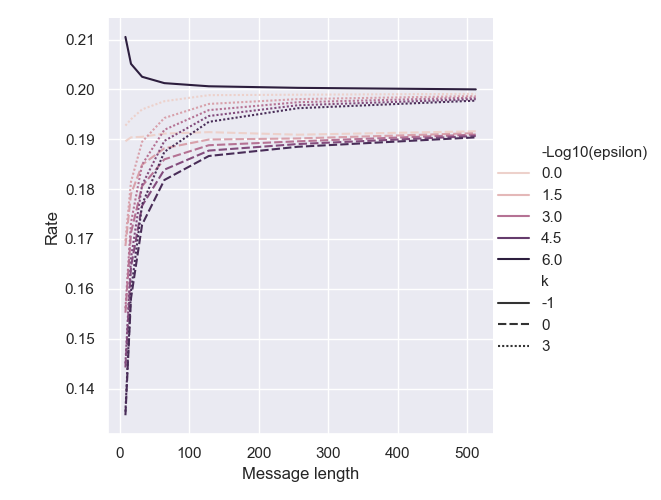
\includegraphics[width=0.35\linewidth]{img/ratep0757q05} &
	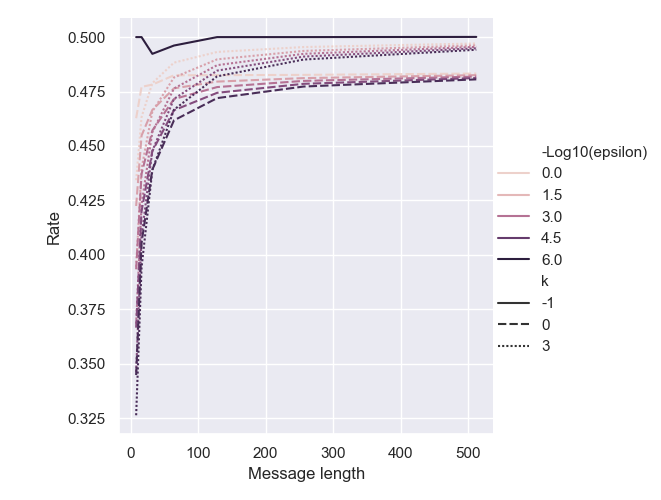
\includegraphics[width=0.35\linewidth]{img/ratep089q09} &
	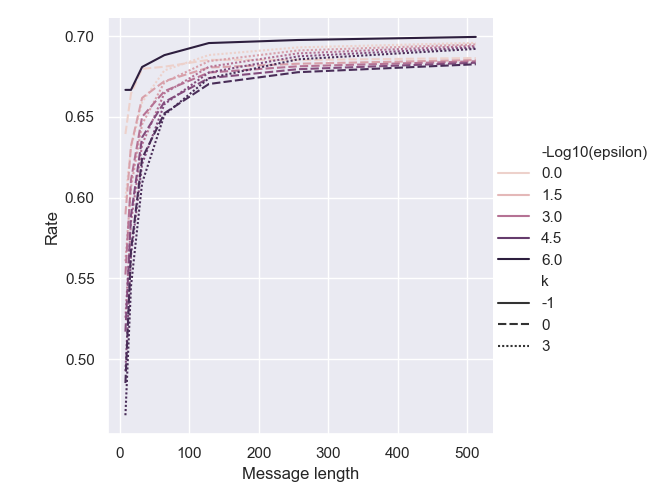
\includegraphics[width=0.35\linewidth]{img/ratep0947q095} \\
	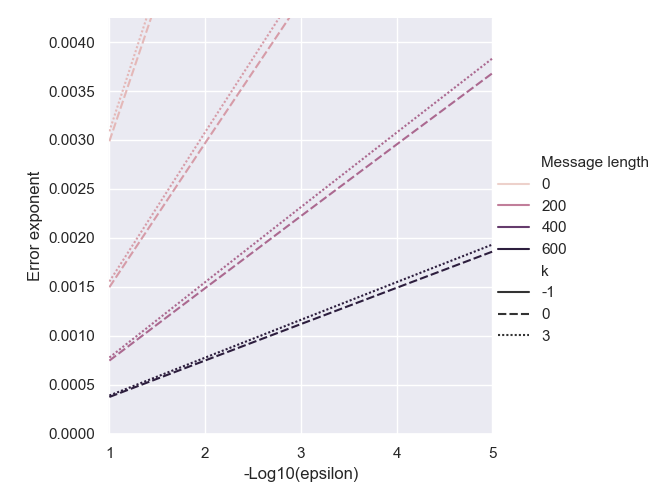
\includegraphics[width=0.35\linewidth]{img/errexp0757q05} &
	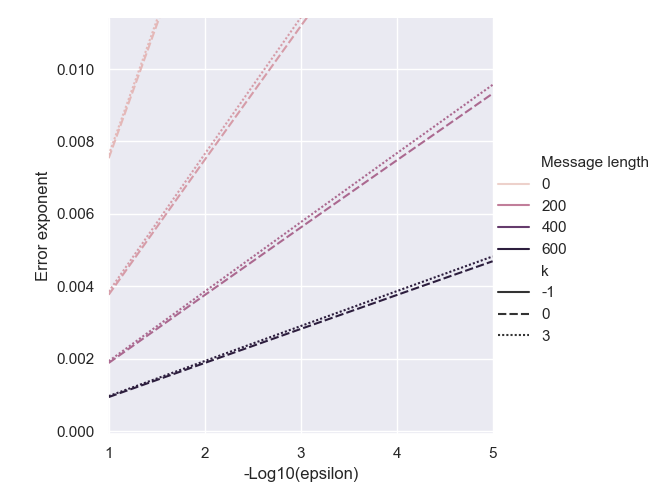
\includegraphics[width=0.35\linewidth]{img/errexp089q09} &
	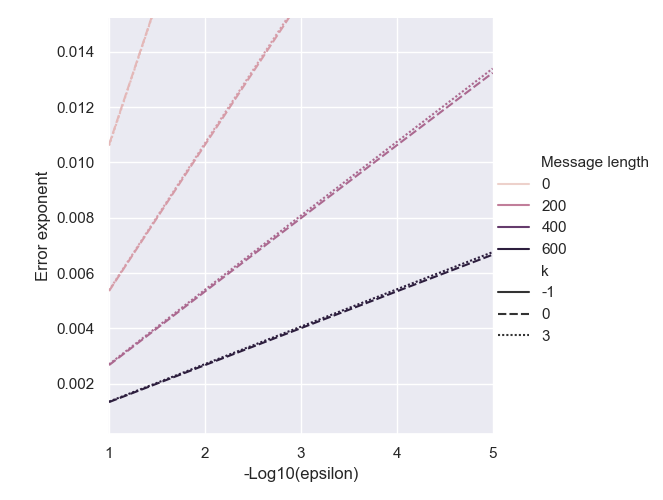
\includegraphics[width=0.35\linewidth]{img/errexp0947q095} \\
	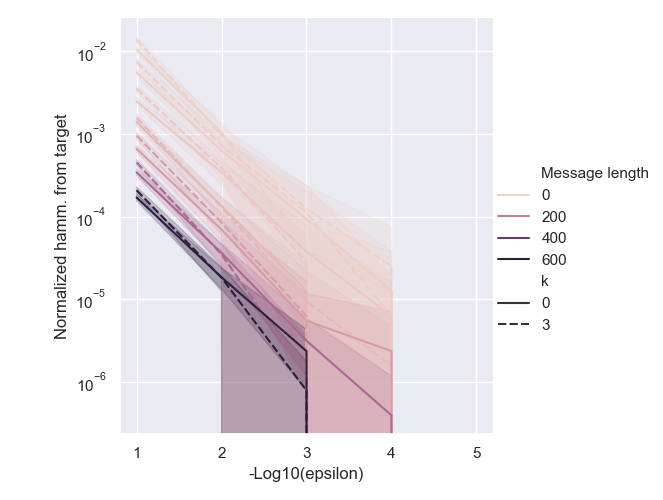
\includegraphics[width=0.35\linewidth]{img/hammp0757q05} &
	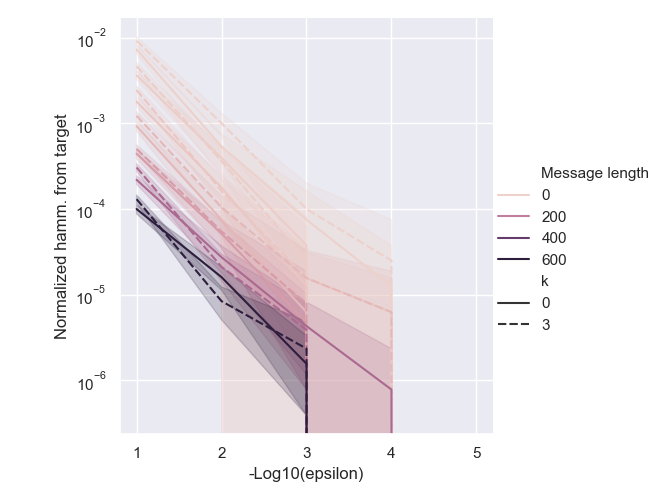
\includegraphics[width=0.35\linewidth]{img/hammp089q09} &
	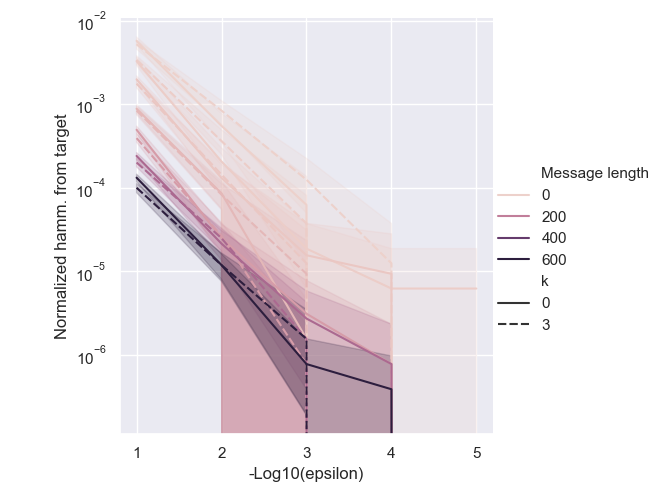
\includegraphics[width=0.35\linewidth]{img/hammp0947q095} \\
		$p=0.757\ (1-H(p)=0.2)$ & $p=0.89\ (1-H(p)=0.5)$ &
		$p=0.947\ (1-H(p)=0.7)$ 
	\end{tabular}
	\captionof{figure}{Finite-length message-decoding results for the
	tree-based causal PBA, with
	$n \in \{8,16,32,64,128,256,512\}$.
	Top row is average convergence rate attained by the algorithm with $k=0$
	(rough dashes) and $k=3$ (fine dashes) as a function
	of $n$, compared to $R(p,q,n)$ (solid). Middle row is error exponent
	for $n \in \{64,128, 256, 512\} $ (darker hues indicate larger $n$)
	as a function of $-\log_{10}\epsilon $.
	All experiments were run for $q$ significantly higher than $1-H(p)$ so
	as to ensure that $R(p,q,n)$ approached $1-H(p)$ very quickly.
	Bottom row is the normalized hamming distance between
	$b_i^*$ and $x_i$ at the time of decoding as a function of
	$-\log_{10}\epsilon$.}
	\label{fig:treegraphs}
\end{figure*}

\subsection{Numeric results for fixed $n$}
Numeric tests were performed over 10000 instances of the implementation, for
message lengths $n \in\{8,16,32,64,128,256,512\}$, decoding thresholds
$1-\epsilon $ such that
$-\log_{10}\epsilon \in \{1,2,3,4,5\}$, and $k\in\{0,3\}$. The prior update
process at each node was approximated using Equation~\ref{eqn:simpapprox}.
The number of steps it took
for the decoder to converge, $\tau$, was recorded for each instance.
The convergence rate $\frac{n}{\mathbb{E}(\tau)}$, error exponent
$\frac{-\log_{10}\epsilon}{\mathbb{E}(\tau)}$, and Hamming distance between
$x_i$ and $b_i^*$ per bit of $b_i^*$ at the time of decoding were
plotted in Figure~\ref{fig:treegraphs}. The normalized hamming distance shows
an exponential decrease as a function of $-\log_{10}\epsilon$. Additionally,
the convergence rate for $k=3$ is shown to asymptotically approach $R(p,q,n)$,
attaining capacity. Code for the tests can be found at~\cite{cataltepecausal}.

\begin{figure*}
	\centering
	\begin{tabular}{ccc}
	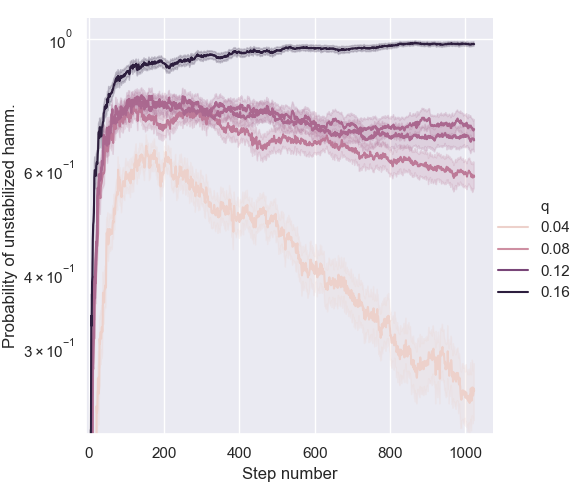
\includegraphics[width=0.35\linewidth]{img/streamingp0684asymptoticqstabilization} &
	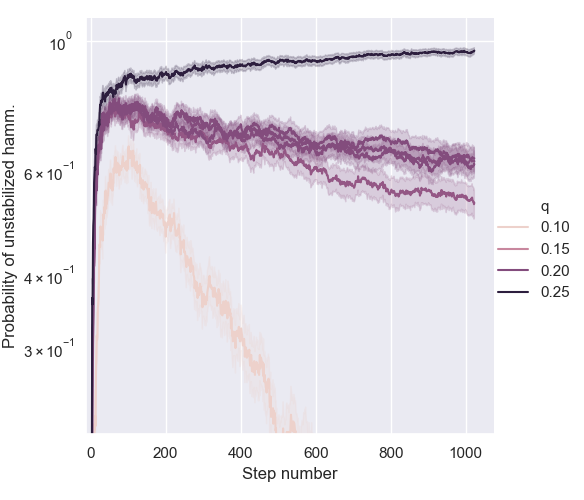
\includegraphics[width=0.35\linewidth]{img/streamingp0757asymptoticqstabilization} &
	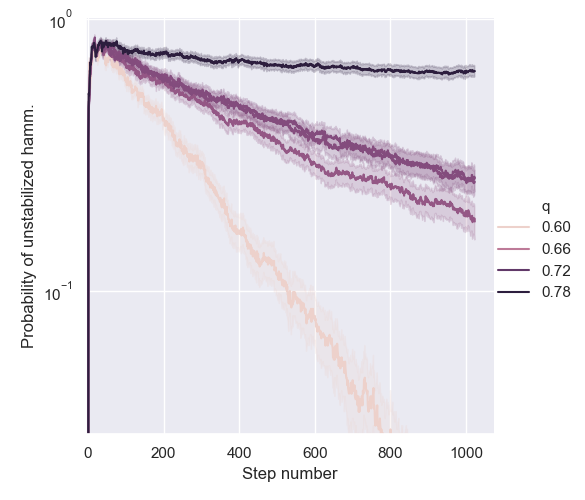
\includegraphics[width=0.35\linewidth]{img/streamingp0947asymptoticqstabilization} \\
$p=0.684$ ($1-H(p)=0.1$) & $p=0.757$ ($1-H(p)=0.2$) & $p=0.947$ ($1-H(p)=0.7$)
	\end{tabular}
	\captionof{figure}{Streaming message-decoding results over 1024 steps
	with 1000 instances of the tree-based causal PBA.
	The $x$-axis in all graphs is the step number.
	The $y$-axis in all graphs is probability that any of the first
	90\% of the bits
	possessed by the encoder and estimated by the decoder at a given step
	are different.
	Darker hues indicate experiments for larger values of $q$, up to
	channel capacity.
	It is seen that the probability of any error in the first
	90\% of bits possessed at a given step decreases exponentially
	as long as $q$ is less than the channel capacity. As $q$ approaches
	channel capacity, we observe that the magnitude of the downward
	slope of decreases until it reaches approximately $0$ when
	$q$ is above channel capacity.}
	\label{fig:treestream}
\end{figure*}
\subsection{Working principles of the algorithm}
The estimate of the algorithm is not necessarily
the mode, but a guess based on the highest-probability
string encountered during a greedy traversal of the tree (this is
due to the fact that it is nontrivial to fully determine the actual mode
from the tree alone
if the current length of the string is not known).
This could
introduce potential disadvantages in accuracy, but this is not reflected
in numeric tests. 

It is likely that the introduction of the predetermined
search limit, which is essentially an estimate of the length of $b_i^*$,
significantly simplifies the problem of searching for the mode by making
it close to the case where one knows the length of the string in advance,
so the estimate found by the tree-based method often ends up being the
mode or close to it.

Additionally, we see that the convergence rate in Figure~\ref{fig:treegraphs}
approaches channel capacity $R(p,q,n)$ for large $n$ 
when $k=3$, but not when $k=0$. It is possible that
for sufficiently large $k$, the algorithm ends up attaining SED at all steps
where it is possible to attain, and thus manages to achieve channel capacity.

\subsection{Numeric results in a streaming setting}
To test the tree-based algorithm's effectiveness in a streaming setting,
the same process was performed as was done for fixed $n$, except $n$ was
set to $1024$ and the algorithm was run for $1024$ steps (i.e., never
reached a terminal node). The parameter $k$ was set to $0$ for all of these
tests. 1000 instances with randomly-generated bits
for $b_i^*$ were
run for each
value of $p$ and $q$, and the
probability of an error in the first $90\%$ of bits
possessed by the encoder and estimated by the decoder was measured. This
quantity is graphed in Figure~\ref{fig:treestream}. For each value
of $p$, we performed experiments with
different values of $q$ approaching the channel capacity.
It was found the probability of error in the leading $90\%$ of bits
displayed an exponential downward trend
right up until $q$ reached channel capacity, at which point it approached
$1$ instead. For the case in Figure~\ref{fig:treestream} where channel capacity
is $0.1$, the magnitude of the slope of the logarithm is very low but still
nonzero right up until $q$ is at channel capacity.
This is expected, as $q$ is the average number of
bits of information that must be sent per transmission for the
Hamming distance between
$b_i^*$ and $x_i$ to be stabilized. Since no more bits of information can
be conveyed per transmission than the channel capacity, the amount of
information the encoder has about a greater proportion of $b_i^*$ will
constantly decrease if $q$ is at or above channel capacity.

\subsection{Disrepancy in performance between fixed $n$ and streaming}
As shown in Figure~\ref{fig:treestream}, the algorithm is able to stabilize
data streamed from a random plant with bit arrival probabilities up to
channel capacity even when $k=0$.
However, results from tests with fixed $n$ shown in
Figure~\ref{fig:treegraphs} show us that the algorithm seems to only
approach $95\%$ of capacity for fixed-length messages when $k=0$.

To measure stabilization in a streaming setting, we measure the probability
of distortion in the leading 90\% of bits received by the encoder and
estimated by the decoder. While this string of bits will, on average, grow
proportionally to the step number, its future-most edge is further and further
in the past as time goes on.
Thus, if we hold the \textit{proportion} (not number)
of bits we are measuring distortion on fixed, the portion of $x_i$ of interest
to us becomes further and further in the past. While this portion of interest
grows proportionally to $i$, it still grows at a rate slower than $q$,
so the decoder receives an increasing
number of bits of information about it.

\section{Conclusions and further work}
We develop a feedback-based error-correcting code in a causal setting where
the encoder receives bits at uniformly random times. Our algorithm uses the
natural tree structure of the space of binary strings to cluster strings and
achieve linear-time performance in numeric tests. We can stabilize a random
plant in a streaming setting with bit arrival rates up to channel capacity.
By adding a constant number
of computations per step, we are able to achieve channel capacity in our rate
of convergence when operating in a setting with a finite-length message.

Future work should concern an analytical assessment of the performance of
this algorithm, as well as numeric tests on different binary-input channels
instead of a BSC.
\bibliography{final}
\bibliographystyle{ieeetr}
\end{document}
